% latex foo.tex 
% dvips -Poutline -G0 foo.dvi -o 
% ps2pdf -dPDFSETTINGS#/prepress foo.ps
\documentclass[]{beamer}
\usepackage{fancyvrb}
\usepackage{tikz}
\usetikzlibrary{arrows}
\tikzset{>=latex}

\newcommand{\myref}[1]{\small\item\url{#1}}
\newcommand{\myreff}[1]{\scriptsize\item\url{#1}}

\newcommand{\mthree}[9]{
\left[
\begin{array}{ccc}
#1 & #2 & #3 \\ #4 & #5 & #6 \\ #7 & #8 & #9
\end{array}
\right]
}

\newcommand{\mrowsix}[6]{
#1 & #2 & #3 & #4 & #5 & #6 
}

\newcommand{\bi}{\begin{itemize}}
\newcommand{\ei}{\end{itemize}}
\newcommand{\sect}[1]{
\section{#1}
\begin{frame}[fragile]\frametitle{#1}
}

\newcommand{\grph}[1]{
\begin{columns}
\column{0.01\textwidth}
\column{0.6\textwidth}
\includegraphics[scale=0.25]{figures/#1.png}
}


\newcommand{\txt}[1]{
\column{0.4\textwidth}
{\parbox{\textwidth}{
\small
\begin{itemize}
#1
\end{itemize}}}
\end{columns}}

\newcommand{\myvec}[1]{
\pstThreeDDot[showpoints=true,drawCoor=true](#1)
\pstThreeDLine[arrows=->,linecolor=blue](0,0,0)(#1)
}


\mode<presentation>
{
%  \usetheme{Madrid}
  % or ...

%  \setbeamercovered{transparent}
  % or whatever (possibly just delete it)
}

\usepackage[english]{babel}

\usepackage[latin1]{inputenc}

\title[Linear Algebra Notes]
{
Linear Algebra Notes
}

%\subtitle{Based on Slides in MIT Open Courseware} % (optional)

\author[Geoffrey Matthews]
{Geoffrey Matthews}
% - Use the \inst{?} command only if the authors have different
%   affiliation.

\institute[WWU/CS]
{
  Department of Computer Science\\
  Western Washington University
}
% - Use the \inst command only if there are several affiliations.
% - Keep it simple, no one is interested in your street address.

\date{Fall 2011}

% If you have a file called "university-logo-filename.xxx", where xxx
% is a graphic format that can be processed by latex or pdflatex,
% resp., then you can add a logo as follows:

\pgfdeclareimage[height=0.5cm]{university-logo}{WWULogoProColor}
\logo{\pgfuseimage{university-logo}}

% If you wish to uncover everything in a step-wise fashion, uncomment
% the following command: 

%\beamerdefaultoverlayspecification{<+->}

\begin{document}


\begin{frame}
  \titlepage
\end{frame}

%\begin{frame}
%  \frametitle{Outline}
%  \tableofcontents
%  % You might wish to add the option [pausesections]
%\end{frame}


\sect{Online Resources}

{\bf Readings}
\begin{itemize}
  \myref{http://chortle.ccsu.edu/vectorlessons/vectorindex.html}
  \myref{http://mathforum.org/mathimages/index.php/Math_for_Computer_Graphics_and_Computer_Vision}
\myref{http://cs229.stanford.edu/section/cs229-linalg.pdf}

\myreff{http://ocw.mit.edu/courses/electrical-engineering-and-computer-science/}, Computer graphics
\myref{http://joshua.smcvt.edu/linearalgebra/}
\end{itemize}
{\bf Videos}
\begin{itemize}
\myref{http://www.khanacademy.org/math/linear-algebra}
\end{itemize}
\end{frame}


\sect{Matrices}
\begin{itemize}
\item A matrix is a set of scalars organized into rows and columns.
\end{itemize}
\[
\left[\begin{array}{cc}
a & b \\
c & d \\
\end{array}
\right]
\]

\end{frame}

\sect{Matrix addition, subtraction, multiplication}
\begin{eqnarray*}
\left[\begin{array}{cc}
a & b \\
c & d \\
\end{array}
\right]
+
\left[\begin{array}{cc}
e & f \\
g & h \\
\end{array}
\right]
&=&\left[\begin{array}{cc}
a+e & b+f \\
c+g & d+h \\
\end{array}
\right]\\
\left[\begin{array}{cc}
a & b \\
c & d \\
\end{array}
\right]
-
\left[\begin{array}{cc}
e & f \\
g & h \\
\end{array}
\right]
&=&\left[\begin{array}{cc}
a-e & b-f \\
c-g & d-h \\
\end{array}
\right]\\
\left[\begin{array}{cc}
a & b \\
c & d \\
\end{array}
\right]
\left[\begin{array}{cc}
e & f \\
g & h \\
\end{array}
\right]
&=&\left[\begin{array}{cc}
ae+bg & af+bh \\
ce+dg & cf+dh \\
\end{array}
\right]
\end{eqnarray*}
\end{frame}

\sect{Multiplication is {\em not} commutative!  $MN \not=NM$}
\begin{eqnarray*}
\left[\begin{array}{cc}
a & b \\
c & d \\
\end{array}
\right]
\left[\begin{array}{cc}
e & f \\
g & h \\
\end{array}
\right]
&=&\left[\begin{array}{cc}
ae+bg & ... \\
... & ... \\
\end{array}
\right]
\\
\left[\begin{array}{cc}
e & f \\
g & h \\
\end{array}
\right]
\left[\begin{array}{cc}
a & b \\
c & d \\
\end{array}
\right]
&=&\left[\begin{array}{cc}
ea+fc & ... \\
... & ... \\
\end{array}
\right]
\end{eqnarray*}
\end{frame}

\sect{Mathematical Vectors}
\begin{eqnarray*}
\vec{v} &=& \left[\begin{array}{c} a\\b\\c \end{array}\right]\\
        &=& [a\  b\  c]^T \\
        &=& (a,b,c)
\end{eqnarray*}
\begin{itemize}
\item A vector is an $N$ row by 1 column matrix.
\item We will use mathematical vectors to represent both {\em points} and {\em vectors} in space.
\end{itemize}
\end{frame}

\sect{Matrices as transforms}
\begin{itemize}
\item{Multiplication of an $N$-vector by an $N\times N$ matrix {\em on the
  left} changes it into another $N$-vector.}
\end{itemize}
\[
\left[\begin{array}{ccc}a&b&c\\d&e&f\\g&h&i\end{array}\right]
\left[\begin{array}{c}x\\y\\z\end{array}\right]
=
\left[\begin{array}{c}x'\\y'\\z'\end{array}\right]
\]
\end{frame}

\sect{Matrix inverses}
\begin{itemize}
\item Identity matrix: \[I=\left[\begin{array}{ccc}1&0&0\\0&1&0\\0&0&1\end{array}\right]\]
\item $AI = IA = A$
\item Some matrices have an inverse: $AA^{-1} = A^{-1}A = I$
\item $(ABC)^{-1} = C^{-1}B^{-1}A^{-1}$
\end{itemize}

\end{frame}

\sect{Determinant of a matrix}
\begin{eqnarray*}
A &=& \left[\begin{array}{cc}
a & b \\
c & d \\
\end{array}\right]\\
\mbox{det}(A) &=&  \left|\begin{array}{cc}
a & b \\
c & d \\
\end{array}\right|\\
&=& ad-bc\\
A^{-1} &=& \frac{\left[\begin{array}{cc}d&-b\\-c&a\end{array}\right]}{\mbox{det}(A)}
\end{eqnarray*}
\end{frame}

\sect{Determinant of a matrix}
\begin{eqnarray*}
\left|\begin{array}{ccc}a&b&c\\d&e&f\\g&h&i\end{array}\right|
&=&
a\left|\begin{array}{cc}e&f\\h&i\end{array}\right|
-b\left|\begin{array}{cc}d&f\\g&i\end{array}\right|
+c\left|\begin{array}{cc}d&e\\g&h\end{array}\right|\\
&=& (aei - afh) - (bdi - bfg) + (cdh - ceg)\\
&=& aei + bfg + cdh - afh - bdi - ceg
\end{eqnarray*}
\end{frame}

\sect{Inverse of a matrix}
\[
\left[\begin{array}{cccccc}a&b&c&1&0&0\\
d&e&f&0&1&0\\
g&h&i&0&0&1\end{array}\right]
\]
\begin{itemize}
\item Stick the identity on the right.
\item Add multiples of one row to another until the identity is on the left.
\item The inverse is now on the right
\end{itemize}
\end{frame}


\sect{Points in Space}

\grph{pointsinspace}

\txt{
\item Points exist in space without a coordinate system.
\item But with only labels it's difficult to compute with them.
}
\end{frame}


\sect{Points in a Coordinate System}

\grph{pointsincoords}


\txt{
\item A coordinate system gives positions to points.
\item Relates {\em points} to {\em tuples of numbers}, or {\em
  mathematical vectors}.  
\item However, points are {\em not} vectors!
}
\end{frame}


\sect{Different Coordinates}
\grph{diffcoord}


\txt{
\item Different coordinate systems give different vectors,
 but the {\em points} are unchanged.
}

\end{frame}


\sect{Physical vectors are differences between points.}

\grph{vectorsarediffs}
\txt{
\item Physical vectors are {\em not} mathematical vectors.
\item But given a coordinate system, you can represent the points as
  mathematical vectors, and then subtract.
\item But these mathematical vectors are not the same thing!
\item Different coordinate systems will give you different
  mathematical vectors for the {\em same} physical vector.
}
\end{frame}

\sect{Points and vectors are not the same thing!}

\grph{vectorsarediffs}
\txt{
\item A point is a position in space.
\item A vector has a magnitude and a direction.
\item The vector from $a$ to $b$ is the point difference:
$\vec{v} = \overrightarrow{ab} = b-a$
\item  You can add two vectors.
\item You {\em cannot} add two points!
\item You can add points and vectors: $b = a+\vec{v} = a + (b-a)$
}
\end{frame}


\sect{Vector Addition}

\grph{vectoraddition}
\txt{
\item vector + vector = vector
\item point + vector = point
\item point - point = vector
\item point + point = {\em nonsense}
}
\end{frame}

\sect{Coordinates give mathematical vectors for physical vectors.}

\grph{coordsgive}
\txt{
\item Subtract the components.
\item $(1,4) - (2,3) = (-1, 1)$
\item $(-1,1) - (2,3) = (-1, -2)$
\item $(1,0) - (2,3) = (-1, -3)$
\item $(4,2) - (2,3) = (2,-1)$
\item Note: we subtract two {\em points} to get a
  {\em vector}. 
}
\end{frame}

\sect{Vectors do not have positions}
\grph{vectorsdonthave}
\txt{
\item Each of these vectors is the {\em same} vector.
}

\end{frame}


\sect{Vectors can be multiplied by scalars}
\grph{vectorsbyscalars}
\txt{
\item Multiplication is repeated addition.
}
\end{frame}


\sect{Lines}
\grph{lines}
\txt{
\item The line through $P$ in the direction $v$ is the set of all
  points $P+\alpha v$ for some $\alpha \in \mathbb{R}$
}
\end{frame}

\sect{Planes (in 3 dimensions)}
\grph{planes}
\txt{
\item The plane through $P$ spanned by $v$ and $w$ is the set of all
  points $P+\alpha v + \beta w$ for some $\alpha,\beta \in \mathbb{R}$
}
\end{frame}



\sect{Affine sums}
\grph{affinesums}
\txt{
\item
$P + \alpha(Q-P)$

$= (1-\alpha)P + \alpha Q$

$= \alpha_1 P + \alpha_2 Q$
\item $\alpha_1 + \alpha_2 = 1$
{\item Think of each point as 
  the vector from some arbitrary point:

${P} \equiv P-O$

${Q} \equiv Q-O$

\item If $0 \leq \alpha_i$ then the point is between $P$ and $Q$.
}}
\end{frame}


\sect{Convex hull}
\grph{convexhull}
\txt{
\item $P= \alpha_1P_1 + \alpha_2P_2 + \ldots + \alpha_nP_n$
\item $\alpha_1 + \alpha_2 + \ldots + \alpha_n = 1$
\item $0 \leq \alpha_i$
}
\end{frame}


\sect{Frames}

\grph{frames}
\txt{
\item A coordinate system can be thought of as a single point, the
  {\em origin}, and a set of {\em basis vectors}.
\item Such a set is called a {\em frame}.
}
\end{frame}


\sect{Frames}
\grph{frames02}
\txt{
\item The coordinates of a point are how many copies of the basis
  vectors you have to add to the origin.
}
\end{frame}


\sect{Frames}
\grph{frames03}
\txt{
\item Note that a frame gives sense to coordinates without anything
  other than points and vectors.
\item A coordinate system is nothing more than an origin and a set of
  basis vectors, a {\em frame}.
\item An {\em orthonormal} frame is one in which all the vectors are
  of unit length and perpendicular to each other.
}
\end{frame}


\sect{Trigonometry}
\grph{trigonometry}
\txt{
\item $\sin(\theta) = o/h$
\item $\cos(\theta) = a/h$
\item $\tan(\theta) = o/a$
}
\end{frame}

\sect{Trigonometry}
\grph{trigonometry02}
\txt{
\item $\tan(\theta) = \sin(\theta)/\cos(\theta)$
}
\end{frame}


\sect{Trigonometry}
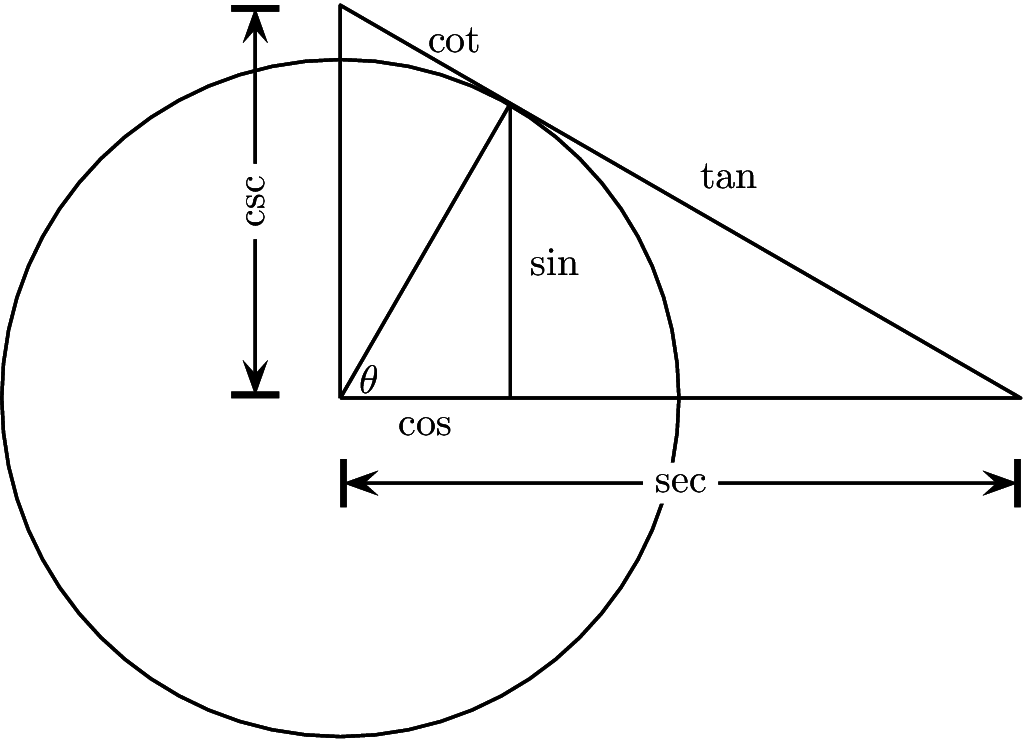
\includegraphics[scale=0.25]{figures/trigonometry03.png}
\end{frame}



\sect{Dot product (Inner product)}
\grph{dotprod}
\txt{
\item $u\cdot v = \cos(\theta)|u||v|$
\pause
\item $|u| = \sqrt{u\cdot u}$
}
\end{frame}


\sect{Projection of one vector on another}
\grph{projection}
\txt{
\item What is $x$?
}
\end{frame}


\sect{Projection of one vector on another}
\grph{projection}
\txt{
\item $x = \cos(\theta)|v|$
\item $x = {u\cdot v}/{|u|}$
}

\end{frame}


\sect{Same direction, opposite direction}
\grph{sameopposite}
\txt{
\item What is the sign of $u\cdot v_i$?
}

\end{frame}


\sect{Same direction, opposite direction}
\grph{sameopposite02}
\txt{
\item Sign of $u\cdot v_i$ 
}
\end{frame}


\sect{{\em AMAZING} theorem about the dot product.}
\begin{itemize}
\item In any coordinate system whatsoever:
\begin{eqnarray*}
u\cdot v &=& (u_x, u_y, u_z)\cdot (v_x, v_y, v_z) \\
&=& u_xv_x + u_yv_y + u_zv_z\\
&=& [u_x\  u_y\  u_z]\left[\begin{array}{c}v_x\\v_y\\v_z\end{array}\right]\\
&=& u^Tv
\end{eqnarray*}
\end{itemize}

\end{frame}

\sect{Example use of the dot product}
\begin{center}
\begin{tikzpicture}
%\draw[help lines] (0,0) grid (8,4);
\draw[thick,*-*] (0,0) node [left] {$q$} -- (8,4) node [right] {$r$};
\draw[thick,*-*] (1,3)  node [left] {$p$};
\draw[thick,dashed,red] (1,3) -- (2,1) node[midway,above] {$x$};
\end{tikzpicture}
\end{center}
\bi
\item An object at $p$ is approaching a wall determined by points $q$ and $r$.
  \item How far away is the wall?
\ei
\end{frame}

\sect{How far away is the wall?}
\begin{center}
\begin{tikzpicture}
%\draw[help lines] (0,0) grid (8,4);
\draw[thick,->] (0,0) node [left] {$q$} -- (8,4) node [right] {$r$} node [midway,below] {$u$};
\draw[thick,->] (0,0)  -- (1,3) node [left] {$p$} node [midway,left] {$v$};
\draw[thick,dashed,red] (1,3) -- (2,1) node [midway,above] {$x$};
\end{tikzpicture}
\end{center}
\bi
\item Let's get some vectors:
  \begin{eqnarray*}
    v &=& p-q\\ u &=& r-q 
\end{eqnarray*}
\item Now what?
\ei
\end{frame}

\sect{How far away is the wall?}
\begin{center}
\begin{tikzpicture}
%\draw[help lines] (0,0) grid (8,4);
\draw[thick,->] (0,0) node [left] {$q$} -- (8,4) node [right] {$r$} node [midway,below] {$u$};
\draw[thick,->] (0,0)  -- (1,3) node [left] {$p$} node [midway,left] {$v$};
\draw[thick,dashed,red] (1,3) -- (2,1) node [midway,above] {$x$};
\draw[thick,dashed,red,xshift=.25em,yshift=-.5em,|-|] (0,0) -- (2,1) node [midway,below] {$y$};
\end{tikzpicture}
\end{center}
\bi
\item Can we find $y$?
\item Will that give us $x$?
\ei
\end{frame}

\sect{How far away is the wall?}
\begin{center}
\begin{tikzpicture}
%\draw[help lines] (0,0) grid (8,4);
\draw[thick,->] (0,0) node [left] {$q$} -- (8,4) node [right] {$r$} node [midway,below] {$u$};
\draw[thick,->] (0,0)  -- (1,3) node [left] {$p$} node [midway,left] {$v$};
\draw[thick,dashed,red] (1,3) -- (2,1) node [midway,above] {$x$};
\draw[thick,dashed,red,xshift=.25em,yshift=-.5em,|-|] (0,0) -- (2,1) node [midway,below] {$y$};
\end{tikzpicture}
\end{center}
  \begin{eqnarray*}
    y &=& \frac{u}{|u|}\cdot v\\
    x &=& \left|p - y\frac{u}{|u|}\right| \\&=& \sqrt{|v|^2 - y^2}
\end{eqnarray*}

\end{frame}

\sect{Cross product (vector product)}
\grph{crossprod}
\txt{
\item A vector at right angles to $u$ and $v$.
\item $u \times v = $\\
$(u_2v_3 - u_3v_2,$\\$ u_3v_1 - u_1v_3,$\\$ u_1v_2 - u_2v_1)$

\item Mnemonic:
\[u\times v = \left|\begin{array}{ccc}
 \vec{i} & \vec{j} & \vec{k} \\
                           u_1 & u_2 & u_3 \\
                           v_1 & v_2 & v_3 \\
\end{array}\right|\]
\item $|u\times v| = |u||v|\sin(\theta)$
}
\end{frame}

\end{document}
